\part{Laboratorio}

\chapter{Introduzione ad Android}

Android è nato nel 2003 come sistema per creare dei dispositivi mobile
avanzati.
\`E stato poi comprato da Google nel 2005 e da allora viene rilasciata
una nuova versione circa ogni anno.

A livello di mercato, Android è stato adottato dalla maggior parte dei
produttori di smartphone e pertanto è installato su più dell'80\% dei
dispositivi.
Questo però comporta un problema a livello di frammentazione:

\begin{itemize}
	\item tanti dispositivi diversi con caratteristiche diverse (schermo, CPU, ecc.)
	\item più versioni del sistema operativo sul mercato in contemporanea in quanto i dispositivi più datati non possono essere aggiornati.
\end{itemize}

Nonostante ciò, il mercato degli smartphone è molto interessante perché è ancora in forte espansione: negli ultimi 3 anni il tempo trascorso per la consultazione di media digitali tramite mobile è più che raddoppiato (figura \ref{lab1-fig-1}), tant'è che lo smartphone è la piattaforma più utilizzata indipendentemente dall'età (figura \ref{lab1-fig-1bis}), fatta eccezione per gli over 65, i quali utilizzano per lo più computer o tablet.
L'utilizzo principale degli smartphone riguarda l'intrattenimento e la comunicazione, con i social network al primo posto come categoria di applicazione più utilizzata (figura \ref{lab1-fig-2}).


\begin{figure}[htbp]
	\centering
	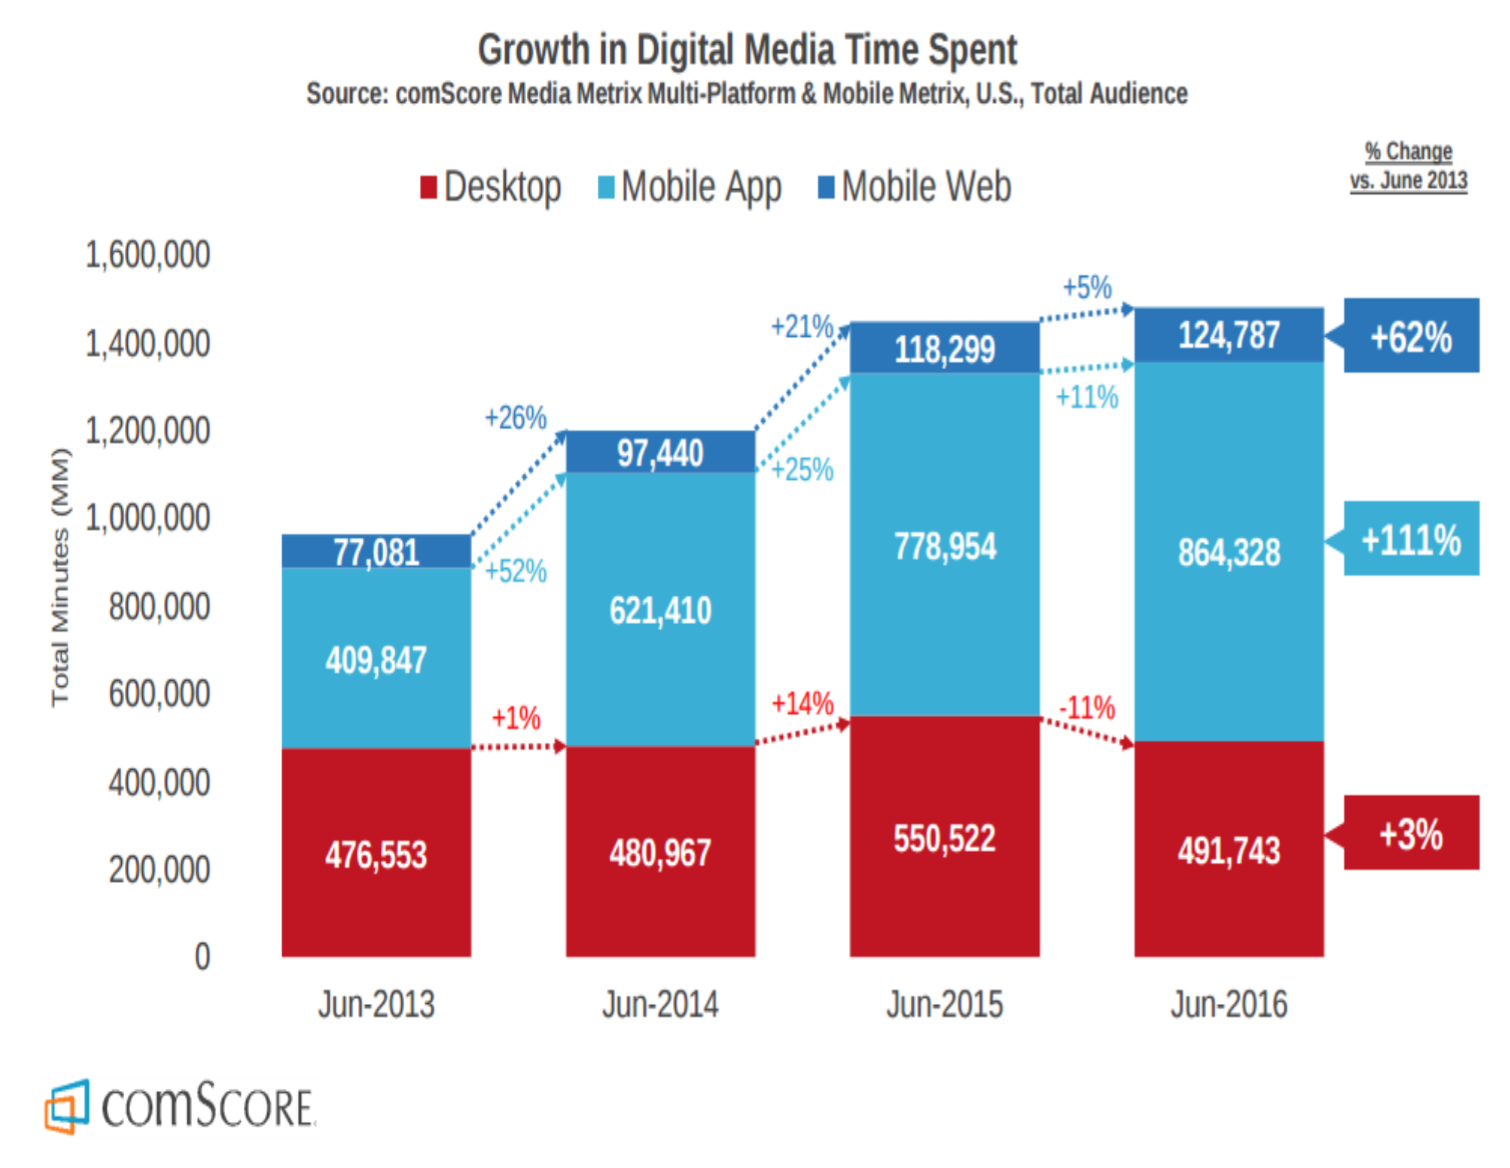
\includegraphics[width=0.8\textwidth]{lab1-fig-1}
	\caption[Crescita del tempo trascorso nella consultazione di contenuti digitali]{Crescita del tempo trascorso nella consultazione di contenuti digitali. Dal grafico si può osservare come gli smartphone siano il fattore trainante della crescita.}\label{lab1-fig-1}
\end{figure}

\begin{figure}[htbp]
	\centering
	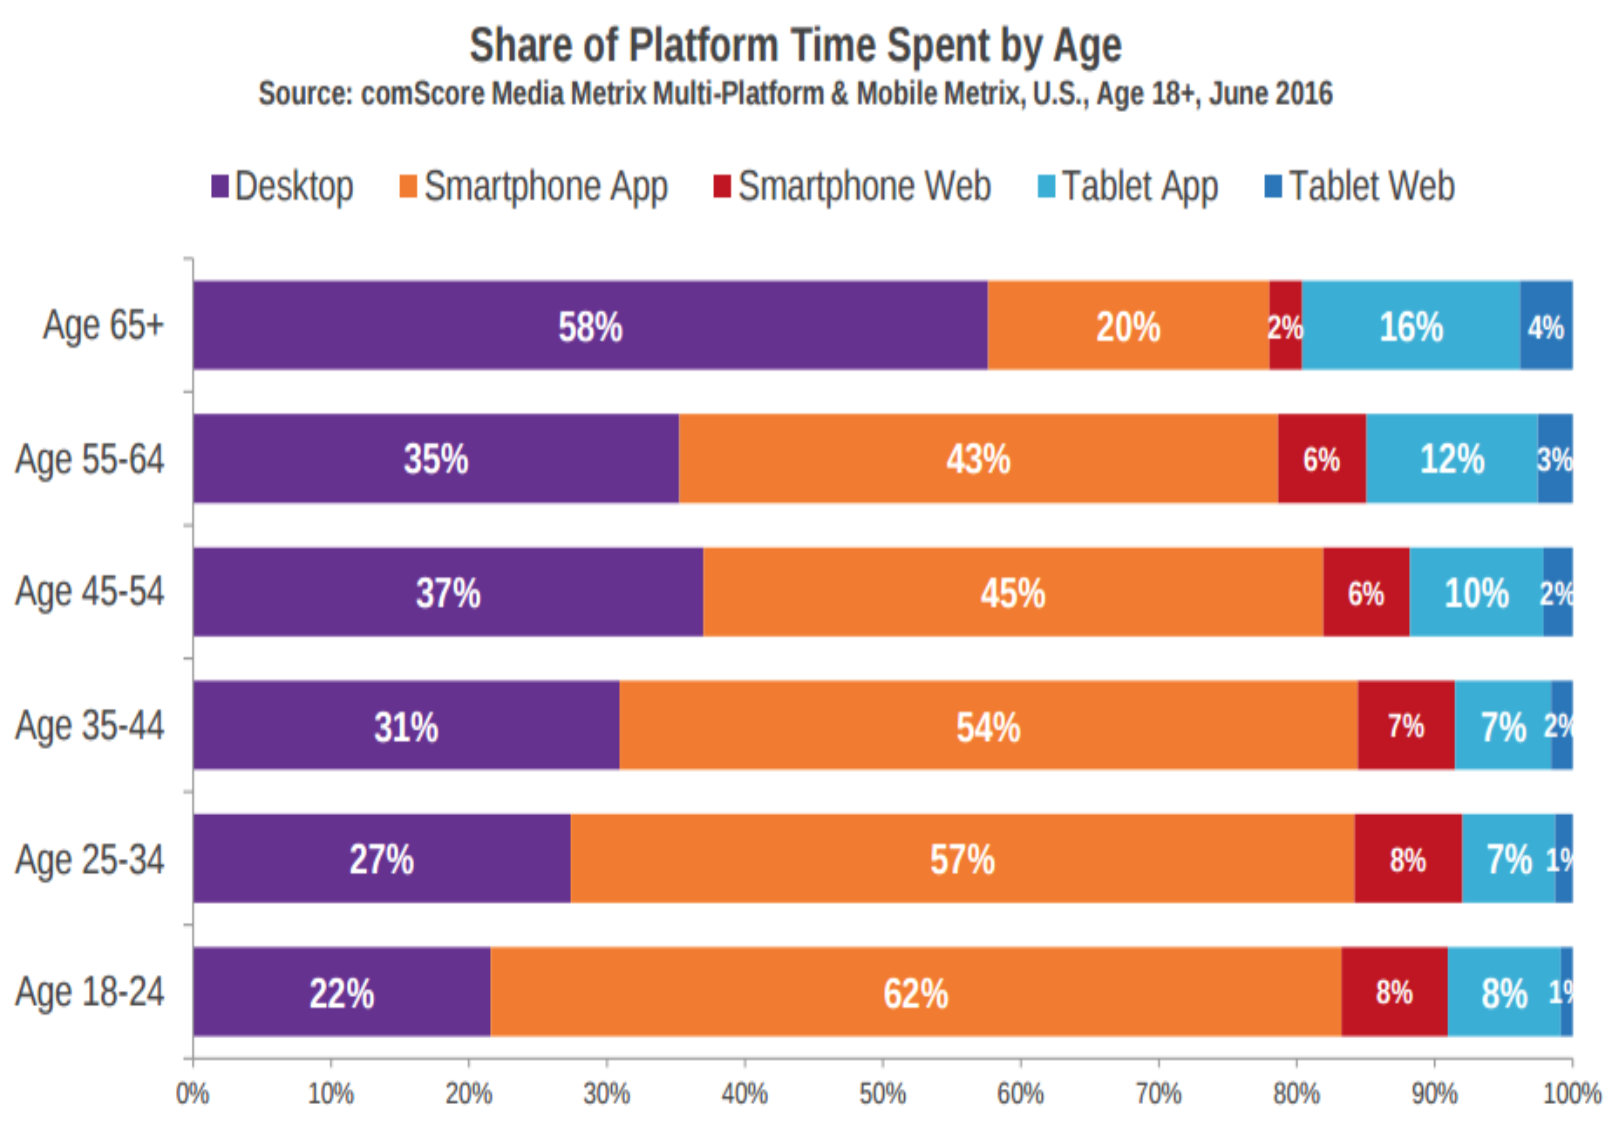
\includegraphics[width=0.8\textwidth]{lab1-fig-1bis}
	\caption[Dispositivi utilizzati al variare dell'età]{Dispositivi utilizzati al variare dell'età. Anche in questo caso lo smartphone risulta essere il più utilizzato per la maggior parte delle fasce d'età.}\label{lab1-fig-1bis}
\end{figure}

\begin{figure}[htbp]
	\centering
	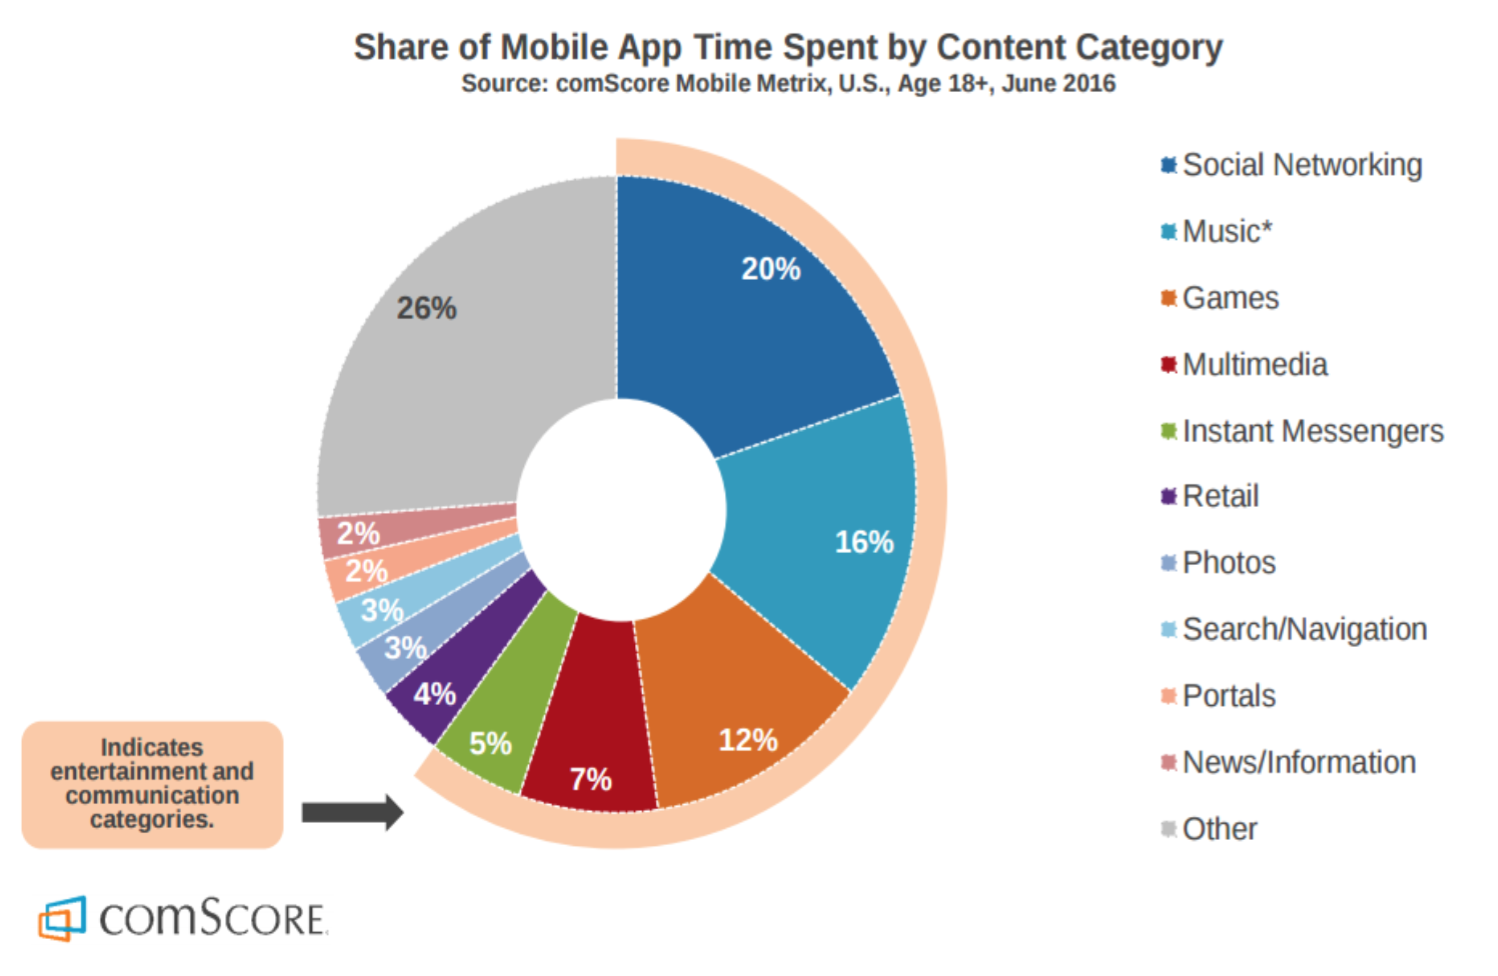
\includegraphics[width=0.8\textwidth]{lab1-fig-2}
	\caption{Tempo d'utilizzo delle applicazioni per smartphone suddiviso per categoria.}\label{lab1-fig-2}
\end{figure}


Per quanto riguarda il come vengono scoperte nuove applicazioni, si ha che iniziano ad essere più efficaci i canali in \textit{push}, in particolare quelli quelli legati alle pubblicità \textit{in-app} e sui social network, anche se la ricerca tramite App Store risulta essere ancora il sistema di scoperta più utilizzato.

Infine, un altro trend importante per le applicazioni mobile riguarda l'accettazione delle notifiche push da parte dell'utente: nell'ultimo anno la percentuale di utenti che non ha concesso il permesso di inviare notifiche ad un'applicazione è passata dal 31\% al 38\%.
Questo aumento può essere dovuto al fatto che è aumentato il numero di applicazioni scaricate da parte dell'utente e che di conseguenza vengano accettate solo le notifiche per le applicazioni che l'utente ritiene importanti.

\section{Architettura di Android}\label{architettura-di-android}

\begin{figure}[htbp]
	\centering
	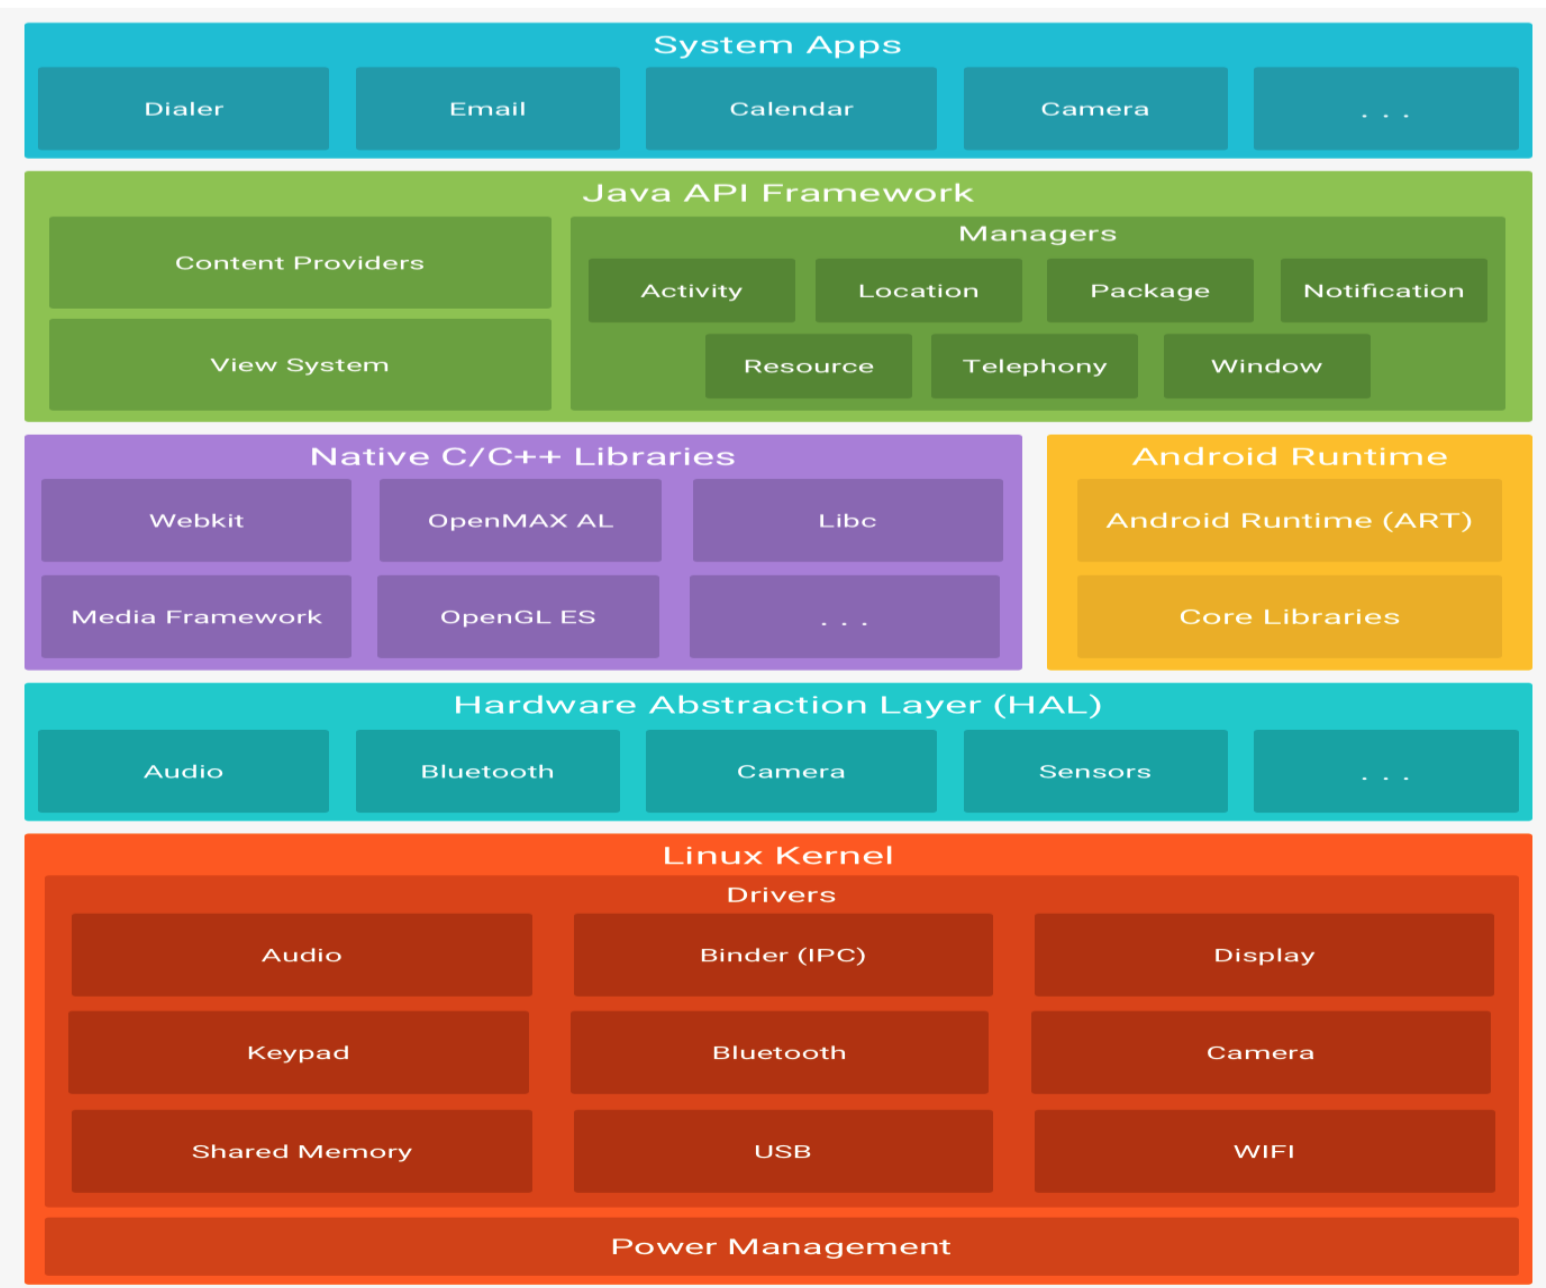
\includegraphics[width=0.8\textwidth]{lab1-fig-3}
	\caption{Architettura a stack di Android.}
\end{figure}

Android si basa su un'architettura a stack:

\begin{itemize}
	\item \textbf{Linux Kernel:} si occupa di gestire la parte di basso livello
		del sistema, rendendo Android facilmente adattabile a vari
		dispositivi. Vengono inoltre ri-utilizzate alcune caratteristiche di
		Linux come l'ambiente per la gestione dei processi e il power
		management. Da notare che Android non è una distribuzione di Linux, ma
		è un sistema operativo a se che utilizza un set ristretto del kernel
		di Linux adatto a funzionare in un ambiente con risorse limitate, il
		quale viene adattato ai vari dispositivi dai rispettivi produttori,
		mantenendo comunque un API comune, in modo che le stesse app possano
		funzionare su dispositivi diversi.
	\item
		\textbf{HAL - Hardware abstraction layer}: effettua un'astrazione
		delle risorse hardware del dispositivo, fornendo un API comune per i
		vari dispositivi.
	\item
		\textbf{Native C++ Libraries:} implementazione delle funzionalità che
		devono essere eseguite in modo efficiente, come il rendering
		dell'interfaccia grafica e dei font, SQLite, ecc.
	\item
		\textbf{Android runtime:} inizialmente utilizzava la Dalvik Virtual
		Machine, un'implementazione della JVM adatta a funzionare con poche
		risorse, con licenza open source e più efficiente della OracleJVM. Le
		applicazioni consistevano quindi una serie di file \texttt{.dex} contenti del
		Bytecode che veniva interpretato dalla VM e che in alcuni casi veniva
		ottimizzato mediante un compilatore just-in-time. A partire da Android
		5.0 la DalvikVM è stata sostituita da \textbf{Android Runtime (ART)},
		un sistema che utilizza tecniche di compilazione \textit{ahead-of-time} per
		tradurre il codice Bytecode (lo stesso che veniva interpretato dalla
		Dalvik VM) in codice nativo. Così facendo il codice nativo deve essere
		prodotto solamente all'installazione dell'applicazione e può essere
		maggiormente ottimizzato, mantenendo la retro-compatibilità con le
		applicazioni esistenti. Lo svantaggio di questo approccio è che
		l'applicazione richiede più memoria per essere installata nel
		dispositivo.
	\item
		\textbf{Java API:} SDK Java per le applicazioni.
	\item
		\textbf{Applicazioni}: app sviluppate utilizzando l'SDK.
\end{itemize}

\begin{figure}[htbp]
	\centering
	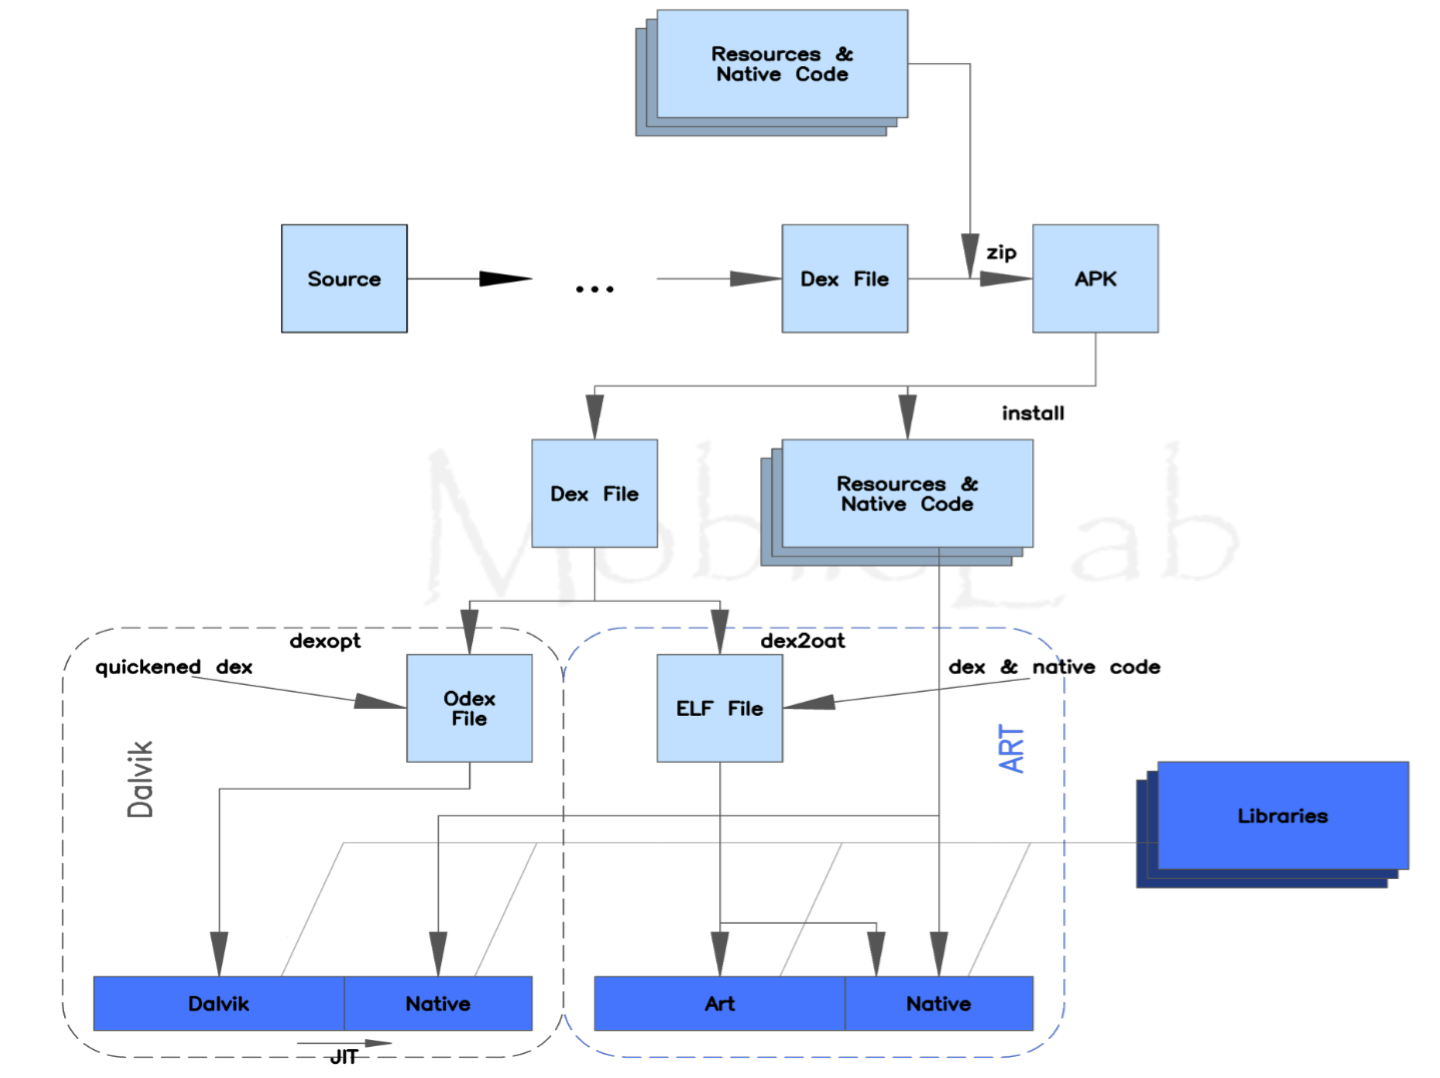
\includegraphics[width=\textwidth]{lab1-fig-3bis}
	\caption[Confronto tra Dalvik e ART]{Confronto tra Dalvik e ART. Con Dalvik, quando viene installato un \texttt{.apk}, il Bytecode contenuto viene trasformato in un Bytecode ottimizzato (\texttt{.odex} file) per poi essere interpretato all'esecuzione dell'applicazione, con delle ottimizzazioni effettuate da un compilatore JIT che traduce dei frammenti di Bytecode in codice nativo. Con ART viene invece compilato il Bytecode in codice nativo (\texttt{.elf} file) in modo che questo possa essere eseguito direttamente, senza passare per un interprete.}
\end{figure}

\section{Android Development Enviroment}\label{android-development-enviroment}

L'ambiente di sviluppo per Android è Android Studio, il quale racchiude
vari tool per gestire l'SDK, un emulatore e altri strumenti utili per il
debug e per la gestione delle librerie.

Un progetto di Android Studio è composto da due componenti principali:

\begin{itemize}
	\item
		\texttt{app} che racchiude tutti gli elementi dell'applicazione. Tra
		questi si trovano:
	\begin{itemize}
		\item \texttt{manifests} contiene il file \texttt{AndroidManifest.xml}, ovvero la
			descrizione dell'applicazione, delle varie \texttt{Activity} e \texttt{Service}, dei
			permessi necessari, ecc.
		\item \texttt{res} contiene tutte le risorse dell'applicazione quali:
			definizioni dei layout delle varie \texttt{Activity}, immagini, costanti e
			stringhe dell'applicazione, ecc.
		\item \texttt{java} contiene il codice dell'applicazione e anche gli
			eventuali test.
	\end{itemize}
	\item \texttt{gradle scripts} che racchiude tutti i file necessari al
		sistema di build Gradle per risolvere le dipendenze e compilare
		l'applicazione.
\end{itemize}

\begin{lstlisting}[language=XML, caption=Esempiod di \texttt{AndroidManifest.xml}]
<?xml version="1.0" encoding="utf-8"?>
<manifest xmlns:android="http://schemas.android.com/apk/res/android"
package="com.manzolik.gmanzoli.mytrains">

	<!-- Esempio di richiesta dei permessi -->
	<uses-permission android:name="android.permission.ACCESS_NETWORK_STATE" />
	<uses-permission android:name="android.permission.INTERNET" />
	
	<!-- Informazioni sull'applicazione -->
	<application
		android:allowBackup="true"
		android:icon="@mipmap/ic_launcher"
		android:label="@string/app_name"
		android:supportsRtl="true"
		android:theme="@style/AppTheme">
		
		<!-- Definizione di un service -->
		<service
			android:name=".services.TrainStatusNotificationService"
			android:exported="false" />
	
		<!-- Activity principale, entry-point dell'applciazione -->
		<activity android:name=".MainActivity">
			<intent-filter>
			<action android:name="android.intent.action.MAIN" />
			
			<category android:name="android.intent.category.LAUNCHER" />
			</intent-filter>
		</activity>
		
		<!-- Altre Activity dell'applicazione -->
		<activity android:name=".TrainStatusActivity" />
		<activity android:name=".EditReminderActivity" />
		<activity android:name=".NoConnectivityActivity" />
		<activity android:name=".FindStationActivity" />
		<activity android:name=".StationStatusActivity" />
	</application>

</manifest>
\end{lstlisting}

Per eseguire un'applicazione è necessario configurare un dispositivo
virtuale utilizzando gli strumenti messi a disposizione da Android
Studio, i quali permettono di simulare varie configurazioni
hardware/software (risoluzione e dimensione dello schermo, sensori
disponibili, versione di Android, ecc.), oppure utilizzare un
dispositivo reale collegato al computer in modalità sviluppatore.

\section{Architettura e funzionamento di un'applicazione}\label{architettura-e-funzionamento-di-unapplicazione}

I componenti principali di un'applicazione Android sono:

\begin{itemize}
	\item \texttt{Activities}: rappresentano un'attività che l'utente può
		effettuare con l'applicazione, tipicamente corrisponde ad una
		schermata dell'applicazione.
	\item \texttt{Fragments}: rappresentano una funzionalità dell'applicazione e
		possono essere utilizzati solo se associati ad un Activity. Vanno a
		definire delle porzioni di interfaccia grafica che vengono
		riutilizzate in più punti dell'applicazione.
	\item \texttt{Services}: programmi che possono eseguire in background e che
		non hanno bisogno di interagire con l'utente.
	\item \texttt{Content Providers}: componenti che permettono di condividere
		dati, sia internamente all'applicazione che con altre applicazioni.
	\item \texttt{Broadcast receivers}: componenti in grado di ricevere delle
		notifiche dal sistema operativo o da altri componenti, come un
		service.
\end{itemize}

L'architettura standard di un'applicazione Android ricorda il pattern
MVC in quanto un \texttt{Activity} funziona sia da \textit{view}, in quanto definisce
l'interfaccia grafica, che da \textit{controller}, in quando incorpora la logica
di gestione degli eventi e di interazione con il Model.

Ogni applicazione viene poi eseguita in un processo Linux appositamente
creato dal sistema operativo quando una porzione di codice
dell'applicazione deve eseguire.

Si ha quindi che il ciclo di vita del processo dell'applicazione è
controllato dal sistema operativo e non dall'applicazione, il quale può
scegliere di terminare o sospendere il processo in base alle sue
necessità.

Android prevede quattro tipologie di processi, che in ordine di priorità
d'esecuzione/risorse sono:

\begin{itemize}
	\item \textbf{Foreground process} è il processo che esegue il codice
		dell'applicazione con la quale sta interagendo l'utente
	\item \textbf{Visible process} è un processo che sta eseguendo del codice il
		cui risultato è visibile all'utente (applicazione attiva ma con
		l'activity in pausa).
	\item \textbf{Service process} è un processo che sta eseguendo un service in
		background.
	\item \textbf{Cached process} è un processo che al momento non è necessario,
		ad esempio perché l'applicazione che sta eseguendo non è visibile
		all'utente.
\end{itemize}

Quando cambia lo stato di un processo di un'applicazione, le varie
activities vengono notificate mediante degli eventi, per i quali lo
sviluppatore può definire dei gestori.

Tali eventi sono:

\begin{itemize}
	\item \texttt{onCreate()} viene sollevato alla creazione dell'\texttt{Activity} e
		viene invocato solamente una volta per tutto il ciclo di vita
		dell'\texttt{Activity}. Tipicamente viene utilizzato per avviare operazioni in
		background e per inizializzare l'interfaccia grafica. Quando
		l'esecuzione è completata, l'\texttt{Activity} non è ancora visibile
		all'utente.
	\item \texttt{onStart()} viene sollevato quando l'\texttt{Activity} sta per diventare
		visibile all'utente. Il gestore dovrebbe configurare il codice di
		gestione dell'UI (listener degli eventi, aggiornamento dei dati
		visualizzati, ecc.).
	\item \texttt{onResume()} viene sollevato quando l'\texttt{Activity} è visibile
		all'utente. Quando l'esecuzione di questo gestore è completata,
		l'utente può interagire con l'\texttt{Activity}, la quale sarà visibile fino a
		quando non si verificherà un'interruzione da parte del sistema o fino
		a quando non verrà visualizzata una nuova \texttt{Activity}. Il gestore
		dovrebbe ri-inizializzare tutte le attività che vengono fermate quando
		l'activity viene messa in pausa.
	\item \texttt{onPause()} viene sollevato quando l'activity ha perso il
		focus, magari a causa della comparsa di una finestra di dialogo, o sta
		per essere nascosta all'utente perché è stata avviata un'altra
		\texttt{Activity}. Il gestore dell'evento dovrebbe essere veloce e dovrebbe
		essere utilizzato per fermare le operazioni CPU-intensive, come le
		animazioni. Da notare che quando viene eseguito il gestore
		l'\textbf{\texttt{Activity} è ancora visibile all'utente}.
	\item \texttt{onStop()} viene sollevato quando l'\texttt{Activity} non è più visibile
		all'utente e il gestore dovrebbe essere utilizzato per rilasciare
		tutte le risorse che non sono più necessarie. Se tutte le activities
		dell'applicazione sono in stato di stop, il processo dell'applicazione
		diventa \emph{cached} e può essere distrutto dal sistema operativo.
		Mentre l'\texttt{Activity} è in stop, lo stato degli oggetti viene mantenuto e
		quindi non è necessario ripristinarlo nel caso l'\texttt{Activity} torni
		visibile.
	\item \texttt{onDestroy()} viene sollevato prima che l'\texttt{Activity} sia
		distrutta. Questo può succedere perché il sistema operativo ha
		distrutto il processo dell'applicazione oppure perché è stato invocato
		il metodo \texttt{finish()} dell'\texttt{Activity}. Il gestore dovrebbe
		assicurarsi che tutte le risorse non rilasciate dell'esecuzione di
		\texttt{onStop} vengano rilasciate. Quando un'\texttt{Activity} viene
		distrutta, il sistema crea in automatico un bundle contenente lo stato
		dell'interfaccia grafica che può essere utilizzato per ripristinare lo
		stato alla successiva creazione dell'\texttt{Activity}.
\end{itemize}

\begin{figure}[htbp]
	\centering
	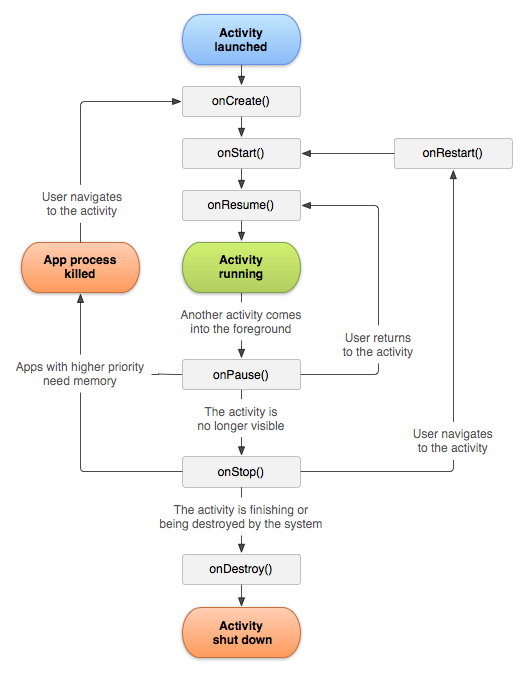
\includegraphics[width=0.7\textwidth]{lab1-fig-4}
	\caption{Ciclo di vita di un \texttt{Activity}}
\end{figure}